\documentclass[11pt]{article}
\usepackage{iftex}
\ifPDFTeX
  \usepackage[T1]{fontenc}
  \usepackage{lmodern}
\fi
\usepackage[margin=1in]{geometry}
\usepackage{graphicx}
\usepackage{amsmath,amssymb}
\usepackage{booktabs}
\usepackage{multirow}
\usepackage{url}
\usepackage[hidelinks]{hyperref}
\usepackage{caption}
\usepackage[section,above]{placeins}
\captionsetup{font=small}

\title{Predict the Breach, Not the Drop:\\Control-Aligned Learning for Smoothing AI Training Power Swings}
\author{Sayed Raheel\\\small\texttt{sayedraheel1995@gmail.com}}
\date{}

\begin{document}
\maketitle

\begin{abstract}
Large AI training jobs move GPU power by tens of percent within a second, and synchronized jobs add
these swings together into fast load ramps of the kind that ramp-rate limits on large loads are meant to
prevent. Fill-type smoothing (filler GPU
work or storage that adds power while the load falls) can remove these violations, but it has to be
engaged before the fall arrives, and keeping it engaged costs energy. A forecaster can decide when to
engage it. We show that what the forecaster is trained to predict matters.
In a matched-pipeline ablation, a gradient-boosted classifier trained on a generic
target, ``a large power drop is coming'', ranks the events a ramp limiter must catch poorly (average
precision, AP, 0.58 on held-out NLR H100 data). Trained on the controller's own event,
``a ramp-limit violation will occur while a limiter triggered now would be engaged'', the same pipeline
reaches AP 0.96 (difference 95\% CI 0.28 to
0.49), against 0.67 for a no-learning rhythm-replay baseline of the same
target. In a limiter simulation with a threshold chosen on validation
data for a 90\% removal target, the learned trigger removes 86.8\% of test violations
with the actuator engaged 45.6\% of the time, while rhythm replay meets the target
only by staying engaged 99.2\% of the time, i.e.\ effectively always on. Across
three public datasets (H100, B200 and V100 nodes; scripted benchmarks and labelled cluster jobs), the learned trigger
ranks violations significantly better than rhythm replay on two datasets when the site is represented in
training (95\% cluster-bootstrap intervals exclude zero); the third is inconclusive. On a site never seen in training, the learned trigger is never
better than rhythm replay in AP, and an hour of local data does not reliably recover the advantage. We
report this as an open problem.
\end{abstract}

\section{Introduction}

Training a large neural network alternates compute-heavy and communication-heavy phases, so GPU power
moves in fast, large steps. Nodes in a synchronized data-parallel job step together, so their power
changes add rather than cancel and the job can look to the grid like one large, fast swing. Industry reports describe swings of tens to hundreds of megawatts and
evaluate software power burning, GPU power floors and rack-level storage as mitigations~\cite{msft_stab}.
Hardware filters and storage that react to the measured load are being developed~\cite{easyrider,
activefilter}; predictive storage control has been studied with perfect preview~\cite{hess} and with
short delay-compensating predictors~\cite{delaycomp}; and AI data center load has been forecast at minute
scales~\cite{stlf}.

This paper studies one specific decision: \emph{when to engage} a fill-type actuator. The actuator (filler
GPU kernels, a battery, a supercapacitor) adds power only while the load falls faster than the allowed
ramp. It must be ready before the fall: kernels must be launched, an inverter must be hot. Readiness has a
cost, so it should be engaged only when needed. A forecaster can make that call. The obvious competitor is
free: training power is periodic, so ``replay the last cycle'' is a strong predictor.

Our contributions are:
\begin{itemize}
\item \textbf{A control-aligned prediction target.} Instead of a generic ``large drop'', the label is the
event the controller acts on: a ramp-limit violation whose whole 1~s ramp window lies inside the window
during which a limiter triggered now would be armed. In a matched-pipeline ablation, retargeting raises AP from 0.58 to 0.96 on held-out NLR
data (Section~\ref{sec:res-target}).
\item \textbf{A readiness analysis} that puts learned triggers, rhythm replay, an always-on limiter and a
perfect-foresight oracle on one curve of violations removed versus time engaged, with operating points
chosen on validation data and scored on test data (Section~\ref{sec:res-ready}).
\item \textbf{A three-dataset study} (H100, B200, V100; scripted benchmarks and labelled cluster jobs) with
cluster-bootstrap confidence intervals, a sensor-harmonization step, and a \textbf{negative result}: a
learned trigger did not transfer to an unseen site (Sections~\ref{sec:res-cross}--\ref{sec:res-unseen}).
\end{itemize}
We are not aware of prior work that studies how the forecasting target affects smoothing performance.

\section{Data}
\label{sec:data}

\begin{table}[t]
\centering
\caption{Datasets. Node-hours are those used for modeling. Units are independent training jobs or sessions; each NLR inference benchmark is one session.}
\label{tab:data}
\footnotesize
\begin{tabular}{@{}l l p{4.2cm} l r r@{}}
\toprule
Dataset & GPUs/node & Workloads & Sensor & Node-h & Units (test) \\
\midrule
NLR~\cite{nlr} & 4$\times$H100 & MLPerf Llama2-70B LoRA, SD; vLLM inference & NVML 5--10 Hz & 248 & 49 (12) \\
Elsayed et al.~\cite{elsayed} & 8$\times$H100 / B200 & diffusion, Llama 1B--8B fine-tuning & NVML & 8 & 32 (6) \\
MIT Supercloud~\cite{supercloud} & 1--2$\times$V100 & 7 model classes, labelled cluster jobs & nvidia-smi 10 Hz & 1,292 & 560 (112) \\
\bottomrule
\end{tabular}
\end{table}

Table~\ref{tab:data} summarizes the three public datasets.

\textbf{NLR}~\cite{nlr} records 4$\times$H100 nodes running MLPerf Llama2-70B LoRA and Stable Diffusion
training on 1 to 16 nodes, plus three vLLM Llama3.1-70B inference benchmarks (offline, online with a
finite request set, online at a fixed rate). We keep at most four nodes per training job; these run
nearly in lockstep and all are weighted equally in the metrics. Training jobs are split whole into train,
validation and test. Each inference benchmark is a single continuous session, cut into one-hour blocks and
split in time; its test blocks therefore count as a single independent cluster, which gives 12 test
clusters in total.

\textbf{Elsayed et al.}~\cite{elsayed} record single 8$\times$H100 and 8$\times$B200 nodes running diffusion
training and Llama 1B--8B fine-tuning sweeps in 15-minute sessions (32 unique sessions).

\textbf{MIT Supercloud}~\cite{supercloud}: we use a stratified subset of 560 labelled jobs, 80 per model
class (VGG, ResNet, Inception, U-Net, BERT, DistilBERT, GNN), on two-V100 nodes (one or two GPU streams
per trace; up to four retained nodes per job, 973 trace segments). These are scheduler-observed jobs on a shared
cluster; the release uses open-source model implementations and public datasets, so they are not
necessarily production workloads, but they are not scripted for power measurement.

\textbf{Common preprocessing.} All traces are averaged onto a 0.2~s grid (row $t$ averages
$[t, t+0.2\,\mathrm{s})$) and expressed as ``NLR-equivalent watts'': node GPU power times 2.8~kW divided by
the node's rated GPU power (2.8~kW for 4$\times$H100, 5.6~kW for 8$\times$H100, 8.0~kW for 8$\times$B200 assuming 1~kW per
B200, and an assumed 250~W per logged V100). We study an illustrative down-ramp threshold of 10\% of rated power per
second, which therefore means the same thing on every node; it is not a specific utility's requirement. Jobs are assigned whole to train, validation and test (about 60/20/20, seed 42). For the
control-aligned models the validation units are split again into two halves: one for early stopping and
one for choosing operating points. For NLR inference, one-hour validation blocks are assigned to these halves after a seeded shuffle;
they come from the same sessions and are not independent.

\textbf{Sensor harmonization.} NVML documents that its default power reading is averaged over a 1~s
interval on Ampere (except GA100) and newer GPUs, which includes the H100 and B200, while on GA100 and
older architectures, including the V100, it returns instantaneous power~\cite{nvml}. The NLR
documentation does not state which reading was logged. Raw V100 traces flicker: without harmonization,
91\% of Supercloud test seconds would be labelled ``violation imminent''. We apply a 1~s trailing mean to
Supercloud so that all three datasets are compared at a similar effective bandwidth. This is an
assumption, discussed in Section~\ref{sec:limits}.

\begin{figure}[t]
\centering
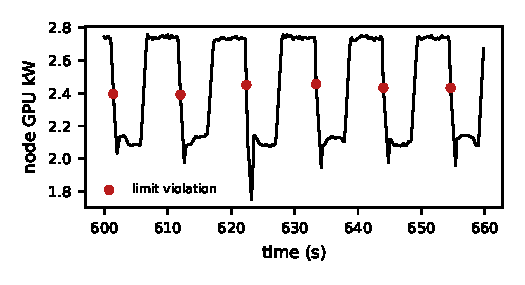
\includegraphics[width=0.6\textwidth]{fig_example.pdf}
\caption{Sixty seconds of one NLR Llama2-70B LoRA test node. Red dots mark exceedances of the illustrative
study threshold (1~s fall larger than 10\% of rated node power). Many are steps of a regular square wave rather than
``big drops''.}
\label{fig:example}
\end{figure}

\section{Problem and methods}
\label{sec:methods}

\subsection{Ramp limit, limiter and readiness}

Let $p_t$ be node power at row $t$ (0.2~s steps) and $F=5$ the number of rows per second. A down-ramp
violation starts at row $v$ when $p_{v-F} - p_v > 0.1\,P_{\mathrm{rated}}$ and this did not hold at $v-1$;
its ramp window is $[v-F, v]$ (Fig.~\ref{fig:example}).

The \emph{limiter} adds power only. When armed, or while still filling, its output is
\begin{equation}
o_t = \max\bigl(p_t,\; o_{t-1} - 0.9\cdot 0.1\,P_{\mathrm{rated}}/F\bigr),
\end{equation}
so it tapers at 90\% of the allowed rate (a safety margin) until it meets the load; otherwise $o_t = p_t$.

A trigger issued at row $t$ acts after a one-row decision delay (row $t$ is complete only at $t+1$) and
an actuator latency $L$ (1~s unless stated), so engagement starts at $e = t + 1 + L F$. Each trigger arms
the limiter for the half-open window $[e, e+H)$ with hold $H$ = 6~s = 30 rows. We count as
\emph{engaged} every row where the limiter is armed or still filling. Performance is the share of raw
violations removed against the share of time engaged. The energy metric is the fill energy plus a standby
draw (we report 0 and 2\% of rated power) while engaged, as a share of job energy. For filler compute this is
extra consumption; for storage it is charge absorbed before any later discharge or loss, which we do not
model.

References: \emph{always-on} (always armed), \emph{always-burn} (a power floor at 80\% of the trailing 60~s peak, which removes only
6.7\% of violations for 6.8\% extra energy), and an \emph{oracle} that arms just in
time for every violation, iterating until violations induced by the limiter itself are also covered.

\subsection{Targets}

The \textbf{big-drop} target labels row $t$ positive if a big-drop onset lies in the next 5~s. An onset
is a row where power falls by more than 30\% of the trailing 10~s peak within the following 1~s, with that
peak at least 1~kW; candidates within 5~s after an onset are merged into it. The \textbf{control-aligned} target labels row $t$ positive if a raw
violation starts at some $v$ with
\begin{equation}
v \in [e + F,\; e + H - 1], \qquad e = t + 1 + LF,
\end{equation}
that is, the whole ramp window $[v-F, v]$ lies inside the armed window $[e, e+H)$. Violations induced by
the limiter itself are not labelled. Many violations are not big drops: the Llama LoRA workload is a
square wave of about 22\% of rated power (Fig.~\ref{fig:example}), so the two targets differ
substantially. We train one model per actuator latency $L \in \{0, 0.2, 0.5, 1, 2, 3\}$~s.

\subsection{Predictors}

\textbf{Rhythm replay} estimates the period $P$ from a trailing 120~s autocorrelation, recomputed every
second: it searches lags of 2 to 40~s, requires a peak correlation of at least 0.3, and takes the first
local peak within 90\% of the strongest (rows with no accepted period score zero). It predicts $\hat p_{t+k} = p_{t+k-P\lceil k/P\rceil}$, and scores row $t$ by the largest predicted
1~s down-ramp whose window lies inside the same target window. It needs no training.

The \textbf{learned} predictor is LightGBM~\cite{lightgbm} on 56 trailing features: current power, lags
and differences over 0.2 to 20~s, rolling mean, standard deviation, minimum and maximum over 1 to 60~s,
time since the last up-step, down-step and drop, autocorrelation and FFT rhythm estimates (period,
strength, phase) and rhythm-replay forecasts at 1, 5 and 10~s. It uses learning rate 0.05, 63 leaves,
at least 200 rows per leaf, 0.8 feature and row subsampling, $\ell_2$ penalty 1, square-root class
weighting, seed 42, and at most 3000 rounds with 100-round early stopping (binary log-loss) on the
early-stopping half of validation. For pooled and leave-one-dataset-out training each dataset receives
equal total sample weight. The earlier big-drop classifier used in the readiness comparisons uses the same
features, 100 rows per leaf, at most 2000 rounds and AP-based early stopping on all validation data; the
matched ablation of Section~\ref{sec:res-target} removes these differences. A \textbf{shape-only} variant, used for transfer, divides every level feature by one watt plus the
trailing 60~s maximum.

\subsection{Evaluation}

NLR models (Sections~\ref{sec:res-target} and \ref{sec:res-ready}) are trained on one row per second
and scored on every 0.2~s row; cross-dataset models (Sections~\ref{sec:res-cross} and
\ref{sec:res-unseen}) are trained and scored on one row per second. Ranking quality is AP on
test rows. Uncertainty is a paired bootstrap over independent clusters
(training jobs; each inference session is one cluster; 1000 resamples). The intervals resample test
clusters for a single fitted model and split; they do not retrain, so they omit training and split
variability. Operating points (thresholds) are chosen on the threshold half of validation and then
scored on test. We call a difference significant when its 95\% interval excludes zero; intervals are
not adjusted for multiple comparisons. For the readiness curves we sweep about 200 thresholds taken from validation-score
quantiles.

\section{Results}

\subsection{The training target}
\label{sec:res-target}

On NLR test traces rhythm replay ranks the control-aligned event with AP 0.67. LightGBM trained
on the control-aligned target reaches 0.96, and the gain over rhythm replay holds for every
workload (Table~\ref{tab:wl}).

\textbf{Matched label ablation.} To isolate the effect of the label, we train the big-drop label through
the same pipeline as the control-aligned model: same training rows, features, fixed LightGBM settings,
early-stopping half, stopping metric and square-root class-weighting rule. Because that rule depends on
label prevalence, the numerical class weight changes with the label (1.75 for the aligned target versus 2.57 for the big-drop target). Scored on the control-aligned event, the
big-drop model reaches AP 0.58 against 0.96 for the aligned model,
a paired cluster-bootstrap difference of 0.37 (95\% CI 0.28 to
0.49, 12 clusters). The big-drop model is not weak at its own task: on the big-drop
event it reaches AP 0.93, where the aligned model reaches only
0.48. The two labels describe different events, and each model is good
at the one it was trained on. (The separately configured big-drop classifier from our earlier pipeline
gives a similar 0.58 on the aligned event.)
The inference workloads are hardest; their falls are dominated by the gaps between benchmark runs.
Results barely depend on actuator latency (Table~\ref{tab:lat}): the regular structure that makes
violations predictable 1~s ahead also makes them predictable 3~s ahead.

\begin{table}[t]
\centering
\begin{minipage}[t]{0.55\textwidth}
\centering
\caption{NLR test AP on the control-aligned target, 1~s latency. Per-workload rows are point estimates;
each inference workload is a single session, so no interval is computed.}
\label{tab:wl}
\small
\begin{tabular}{@{}lcc@{}}
\toprule
Workload & Learned & Rhythm replay \\
\midrule
Llama2-70B LoRA training & 1.00 & 0.81 \\
Stable Diffusion training & 0.96 & 0.73 \\
Offline inference & 0.55 & 0.29 \\
Online inference, finite & 0.76 & 0.09 \\
Online inference, fixed rate & 0.65 & 0.36 \\
\midrule
All & 0.96 & 0.67 \\
\bottomrule
\end{tabular}
\end{minipage}\hfill
\begin{minipage}[t]{0.4\textwidth}
\centering
\caption{NLR test AP by actuator latency.}
\label{tab:lat}
\small
\begin{tabular}{@{}rcc@{}}
\toprule
$L$ (s) & Learned & Rhythm \\
\midrule
0 & 0.96 & 0.68 \\
0.2 & 0.96 & 0.68 \\
0.5 & 0.96 & 0.68 \\
1 & 0.96 & 0.67 \\
2 & 0.96 & 0.67 \\
3 & 0.95 & 0.67 \\
\bottomrule
\end{tabular}
\end{minipage}
\end{table}

\subsection{Readiness on NLR}
\label{sec:res-ready}

Fig.~\ref{fig:ready} sweeps each trigger's threshold on NLR test traces. Every trigger can reach high
removal by staying engaged long enough; what differs is how much engaged time it needs.

\textbf{Validation-chosen operating points} are the deployable result (Table~\ref{tab:ops}). For a 90\%
removal target, the learned control-aligned trigger removes 86.8\% of test violations
at 45.6\% engaged time, slightly short of target. Rhythm replay reaches
99.8\% only by staying engaged 99.2\% of the time,
which is the always-on solution. With a 2\% standby draw the reported energy metrics are
3.7\% and 5.4\% (always-on: 5.4\%).
At an 80\% target both triggers undershoot on test (73.7\% and
74.4\%): thresholds chosen on a few validation jobs transfer imperfectly. The
perfect-foresight oracle removes all violations at 29.8\% engaged time. It is an iterative
just-in-time heuristic rather than a proven minimum, but it indicates how much better prediction could
still gain.

\begin{table}[t]
\centering
\caption{Validation-chosen operating points scored on NLR test traces (1~s latency). Removal and engaged
time in \%; reported energy metric in \% of baseline job energy with a 2\% standby draw.}
\label{tab:ops}
\small
\begin{tabular}{@{}llccc@{}}
\toprule
Target & Trigger & Removed & Engaged & Energy metric \\
\midrule
\multirow{3}{*}{80\%} & Learned, aligned & 73.7 & 35.9 & 2.9 \\
 & Rhythm, aligned & 74.4 & 43.3 & 3.2 \\
 & Learned, big-drop & 88.0 & 61.4 & 4.3 \\
\midrule
\multirow{3}{*}{90\%} & Learned, aligned & 86.8 & 45.6 & 3.7 \\
 & Rhythm, aligned & 99.8 & 99.2 & 5.4 \\
 & Learned, big-drop & 92.7 & 69.1 & 4.6 \\
\midrule
\multirow{3}{*}{95\%} & Learned, aligned & 91.6 & 49.7 & 4.0 \\
 & Rhythm, aligned & 99.8 & 99.2 & 5.4 \\
 & Learned, big-drop & 95.4 & 75.8 & 4.8 \\
\midrule
 & Always-on & 100.0 & 100.0 & 5.4 \\
 & Oracle & 100.0 & 29.8 & 3.6 \\
\bottomrule
\end{tabular}
\end{table}

\textbf{Attainable trade-offs (retrospective).} Table~\ref{tab:arm} reads, from each test curve, the least
engaged time at which a removal level is reached. Because the threshold is picked on test, this compares
attainable trade-offs rather than deployable operating points. To remove 90\% of violations the learned
control-aligned trigger needs 48.4\% engaged time and rhythm replay
99.2\%: a paired cluster-bootstrap difference of $-$50.8
points (95\% CI $-$57.4 to $-$8.8). The interval is
asymmetric because the statistic is a minimum over thresholds: in most resamples rhythm replay needs more
than 95\% engagement, but some cluster mixtures cross 90\% removal at 50--80\%. At 95\% removal the
difference is $-$40.8 points (CI $-$49.1 to
$-$31.4). Against the learned big-drop trigger the difference is
$-$15.9 points at 90\% (CI $-$25.7 to $-$3.9)
but not significant at 95\% (CI $-$26.3 to 0.5); with 12 test
clusters the effect of the target is clearest in ranking quality.

\begin{table}[t]
\centering
\caption{Retrospective: least engaged time (\%) on the NLR test curve that reaches each removal level,
1~s latency. Thresholds are read off the test curve.}
\label{tab:arm}
\small
\begin{tabular}{@{}lccc@{}}
\toprule
Removal & Learned, aligned & Rhythm, aligned & Learned, big-drop \\
\midrule
80\% & 43.1 & 51.5 & 53.0 \\
90\% & 48.4 & 99.2 & 64.3 \\
95\% & 58.4 & 99.2 & 74.8 \\
\bottomrule
\end{tabular}
\end{table}

\begin{figure}[t]
\centering
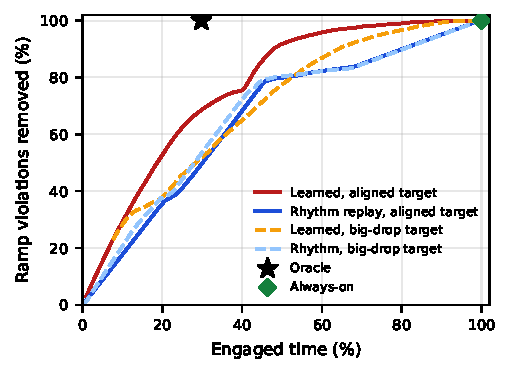
\includegraphics[width=0.6\textwidth]{fig_readiness.pdf}
\caption{Violations removed versus engaged time on NLR test traces (1~s latency, about 200 thresholds from
validation-score quantiles). Always-on removes everything but is always engaged; the star is the iterative
perfect-foresight oracle.}
\label{fig:ready}
\end{figure}

\subsection{Across sites and GPUs}
\label{sec:res-cross}

Table~\ref{tab:cross} and Fig.~\ref{fig:forest} compare AP in three configurations: trained on the test
site's own training jobs (in-domain), trained on all three datasets (pooled), and trained on the other two
only (unseen site). In-domain or pooled, the learned trigger ranks violations significantly better than
rhythm replay on NLR and on Supercloud. On Supercloud, exploratory per-class intervals (not
corrected for multiplicity) are positive for 7 of 7 model classes. On
Elsayed the point estimate favours learning but the interval includes zero with only six test sessions,
and rhythm replay is better on its two diffusion test sessions; their very regular cadence may suit
replay, but two sessions do not allow a firm conclusion.

\begin{table}[t]
\centering
\caption{Test AP, learned versus rhythm replay, with the 95\% cluster-bootstrap interval of the
difference. Unseen site uses the ordinary features (shape-only results in Table~\ref{tab:transfer}).}
\label{tab:cross}
\small
\begin{tabular}{@{}llccc@{}}
\toprule
Test dataset & Training data & Learned & Rhythm & Difference CI \\
\midrule
\multirow{3}{*}{NLR} & in-domain & 0.96 & 0.67 & [0.22, 0.36] \\
 & pooled & 0.96 & 0.67 & [0.22, 0.37] \\
 & unseen site & 0.53 & 0.67 & [$-$0.23, $-$0.02] \\
\midrule
\multirow{3}{*}{Supercloud} & in-domain & 0.88 & 0.74 & [0.11, 0.19] \\
 & pooled & 0.88 & 0.74 & [0.11, 0.18] \\
 & unseen site & 0.68 & 0.74 & [$-$0.10, $-$0.02] \\
\midrule
\multirow{3}{*}{Elsayed} & in-domain & 0.93 & 0.88 & [$-$0.11, 0.09] \\
 & pooled & 0.92 & 0.88 & [$-$0.13, 0.08] \\
 & unseen site & 0.84 & 0.88 & [$-$0.43, 0.05] \\
\bottomrule
\end{tabular}
\end{table}

\begin{figure}[t]
\centering
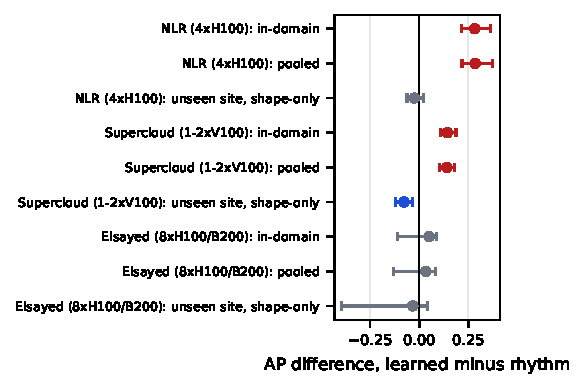
\includegraphics[width=0.6\textwidth]{fig_forest.pdf}
\caption{AP difference, learned control-aligned trigger minus rhythm replay, with 95\% cluster-bootstrap
intervals. Red: learned significantly better; blue: rhythm significantly better; grey: inconclusive. The
unseen-site rows use shape-only features.}
\label{fig:forest}
\end{figure}

AP is a ranking measure, not a smoothing result. Table~\ref{tab:xready} reports validation-chosen
operating points for a 90\% removal target on each dataset (one decision per second, no confidence
intervals). The learned trigger lands below target on Elsayed and slightly below on the others; rhythm
replay meets the target on NLR and Supercloud only by staying engaged almost all the time, and misses it
on Elsayed. On NLR and Supercloud learning therefore trades about 12 points of removal for roughly half
the engaged time; on Elsayed it removes more at similar engaged time. Without intervals these comparisons
are descriptive.

\begin{table}[t]
\centering
\caption{Validation-chosen operating points for a 90\% removal target, scored on test (pooled training;
one decision per second). Removed / engaged, in \%.}
\label{tab:xready}
\small
\begin{tabular}{@{}lcc@{}}
\toprule
Test dataset & Learned & Rhythm replay \\
\midrule
NLR & 88.2 / 44.0 & 99.8 / 99.1 \\
Supercloud & 87.7 / 53.6 & 99.8 / 99.3 \\
Elsayed & 83.4 / 55.4 & 67.3 / 51.8 \\
\bottomrule
\end{tabular}
\end{table}

\subsection{Unseen sites}
\label{sec:res-unseen}

When the test dataset is excluded from training, the learned trigger is not better than rhythm replay in
AP on any dataset, and with the ordinary features it is significantly worse on NLR and Supercloud
(Table~\ref{tab:cross}). Absolute power levels differ across GPU generations even after normalization, so
we tried two remedies (Table~\ref{tab:transfer}). Shape-only features close the NLR gap to an
inconclusive difference but remain significantly worse on Supercloud. Continuing to boost the unseen-site
model on 5, 15 or 60 minutes of the new site's training data (mean and range over five random draws)
does not reliably recover the in-domain advantage (a draw is left unadapted if its local fitting subset
or its early-stopping tail contains only one class). Rhythm replay needs no site data to score, only to set a
threshold; in our experiments a learned trigger needed the site in its training set to rank better.

Validation-chosen operating points tell a slightly different story, but they are not fully zero-shot:
the thresholds of both triggers are chosen on the held-out site's own validation data, so ``unseen''
refers to model fitting only. With ordinary features, the unseen-site learned trigger on NLR removes 90.3\% of violations at
58.0\% engaged time, against 99.8\% at
99.1\% for rhythm replay. Ranking quality and engaged time can therefore
disagree; we have no interval for this comparison and do not claim transfer from it.

\begin{table}[tb]
\centering
\caption{Transfer to an unseen site with shape-only features. Adapted rows: mean (range) AP over five
draws of local data. Rhythm replay AP for reference.}
\label{tab:transfer}
\small
\begin{tabular}{@{}lccc@{}}
\toprule
 & NLR & Supercloud & Elsayed \\
\midrule
Rhythm replay & 0.67 & 0.74 & 0.88 \\
In-domain, shape-only & 0.96 & 0.88 & 0.88 \\
Unseen site, shape-only & 0.65 & 0.66 & 0.85 \\
\quad difference CI & [$-$0.06, 0.02] & [$-$0.12, $-$0.04] & [$-$0.39, 0.04] \\
+ 5 min of site data & 0.63 (0.56--0.65) & 0.62 (0.59--0.66) & 0.82 (0.76--0.85) \\
+ 15 min & 0.59 (0.55--0.65) & 0.64 (0.57--0.67) & 0.78 (0.66--0.88) \\
+ 60 min & 0.71 (0.62--0.77) & 0.64 (0.58--0.69) & 0.84 (0.80--0.91) \\
\bottomrule
\end{tabular}
\end{table}

\section{Discussion and limitations}
\label{sec:limits}

\textbf{Why the target matters.} The big-drop label teaches the model about one kind of event (large
falls) at one horizon (the next 5~s). The limiter needs something else: a fall steep enough to break the
ramp limit, inside the window its own latency and hold time define. Many violations, such as the steps
of the LoRA square wave, never qualify as big drops, so a big-drop model never learns to rank them. In the
matched ablation all fixed pipeline choices and the class-weighting rule are held constant; the label and
its prevalence-derived class weight change together, so the gap is attributable to the choice of training
target (Section~\ref{sec:res-target}).

\textbf{Why rhythm replay is always on at high removal.} Replay predicts each violation from the previous
cycle. Violations that do not repeat (phase changes, gaps between inference runs) score near zero, so the
only way for replay to catch them is to lower the threshold until the limiter is armed almost all the
time.

\textbf{Limitations.}
\emph{Sensors.} If NLR and Elsayed power is NVML's 1~s average, true ramps are faster than measured and
measured lead times are optimistic; harmonizing Supercloud with a 1~s mean is an assumption.
\emph{Uncertainty.} Intervals are conditional on one fitted model and one split and do not include
training or split variability; NLR has 12 test clusters and Elsayed six. Up to four near-synchronous nodes
per NLR job, and up to four retained nodes per Supercloud job, are weighted equally, and metrics pool rows, so longer and larger
jobs weigh more in point estimates; the bootstrap resamples whole jobs but does not change this
weighting. For NLR inference, the two
validation halves are not independent.
\emph{Simulation.} The actuator is an idealized one-sided limiter with fixed latency, hold time and
standby draw. Actuator power limits, storage capacity, state of charge, later discharge, efficiency,
wear and measured actuator dynamics are not modelled, and the standby cost is an assumed fraction of rated
power. The ramp threshold is illustrative and applied per node.
\emph{Workloads.} NLR and Elsayed are scripted benchmarks; NLR inference falls are dominated by gaps
between benchmark runs, and each NLR inference workload is a single session. Supercloud adds scheduler-observed cluster
jobs, but on older V100 nodes.
\emph{Scale.} All results are per node. Synchronized multi-node jobs scale the same swing, while
desynchronized jobs partly cancel; we do not model facility-level aggregation.

\textbf{Future work.} Repeated whole-job splits or a nested bootstrap that retrains; one-node-per-job
sensitivity; a storage model with state of charge; and methods that let a learned trigger transfer to a
new site, or at least decide quickly whether to fall back to rhythm replay.

\section{Conclusion}

For fill-type smoothing of AI power swings, a forecaster should be trained on the controller's event, a
ramp-limit violation inside the actuator's engagement window, rather than on a generic large drop. With
that target, a small gradient-boosted model needs substantially less engaged time than rhythm replay for
the same violation removal on H100 benchmark traces (retrospectively, with thresholds read off the test
curve; Table~\ref{tab:arm}), and ranks violations better (higher AP) on V100
cluster jobs, provided the site is represented in training. Closing the gap to the oracle and making learned
triggers transfer to new sites are the natural next steps.

\section*{Data, code and licences}
The NLR data are released under the National Laboratory of the Rockies dataset licence, which permits
use with attribution. The Elsayed et al.\ dataset is listed as CC~BY~4.0 on figshare, while the README
inside its archive states CC~BY-NC-ND; we treat it conservatively as non-commercial. The MIT Supercloud
data are CC~BY-NC-ND~4.0. All three are used for research only and none is redistributed; readers can
obtain them from the original sources. The reported model and controller metrics are generated from result tables written by the analysis
pipeline. The code is available from the author on request.

\section*{Use of AI tools}
Analysis code and text were drafted with the help of AI coding and writing assistants and independently
reviewed by a separate AI model. The author checked the results and is responsible for the content.

\begin{thebibliography}{99}
\bibitem{msft_stab} E.~Choukse, B.~Warrier, S.~Heath, et al., ``Power stabilization for AI training datacenters,'' arXiv:2508.14318, 2025.
\bibitem{easyrider} D.~Jensen, G.~Wilkins, O.~Nnorom~Jr., H.~Budd, R.~Rajagopal, J.~Rivas-Davila, and P.~Levis, ``EasyRider: Mitigating power transients in datacenter-scale training workloads,'' arXiv:2604.15522, 2026.
\bibitem{activefilter} D.~Jensen, G.~Wilkins, O.~Nnorom~Jr., H.~Budd, P.~Levis, and J.~Rivas, ``Active filter design for buffering datacenter-scale power fluctuations from training AI,'' arXiv:2609.13490, 2026.
\bibitem{hess} H.~You, C.~Lou, and J.~Yang, ``Source side mitigation of AI datacenter power fluctuations with a hybrid energy storage system and residual differentiable predictive control,'' arXiv:2606.04869, 2026.
\bibitem{delaycomp} X.~Lyu, W.~Du, S.~M.~Mohiuddin, and B.~A.~Ross, ``Communication delay robust control of BESS for AI training load smoothing,'' arXiv:2609.22542, 2026.
\bibitem{stlf} M.~Mughees, Y.~Li, Y.~Chen, and Y.~R.~Li, ``Short-term load forecasting for AI-data center,'' arXiv:2503.07756, 2025 (accepted to IEEE PES General Meeting 2025).
\bibitem{nlr} R.~Vercellino, J.~Willard, G.~Campos, W.~da~Silva~Pereira, O.~Hull, M.~Selensky, and J.~Mueller, ``Measurement of generative AI workload power profiles for whole-facility data center infrastructure planning,'' arXiv:2604.07345, 2026. Data: ``Dataset of Generative AI Workload Power Profiles,'' National Laboratory of the Rockies, doi:10.7799/3025227.
\bibitem{elsayed} A.~A.~E.~Elsayed, A.~A.~Al-Obaidi, and H.~E.~Z.~Farag, ``Characterization of high-resolution AI data center training workloads on single and multiple GPU nodes,'' \emph{Scientific Data}, vol.~13, art.~1268, 2026, doi:10.1038/s41597-026-07496-6. Data: figshare, doi:10.6084/m9.figshare.31654879.
\bibitem{supercloud} S.~Samsi, M.~L.~Weiss, D.~Bestor, et al., ``The MIT Supercloud dataset,'' in \emph{Proc. IEEE High Performance Extreme Computing Conf. (HPEC)}, 2021, pp.~1--8, doi:10.1109/HPEC49654.2021.9622850.
\bibitem{nvml} NVIDIA, ``NVML API reference: nvmlDeviceGetPowerUsage,'' \url{https://docs.nvidia.com/deploy/nvml-api/api/group__nvmlDeviceQueries.html}, accessed 2026-10-15.
\bibitem{lightgbm} G.~Ke, Q.~Meng, T.~Finley, T.~Wang, W.~Chen, W.~Ma, Q.~Ye, and T.-Y.~Liu, ``LightGBM: A highly efficient gradient boosting decision tree,'' in \emph{Advances in Neural Information Processing Systems}, vol.~30, 2017.
\end{thebibliography}

\end{document}
